\documentclass[a4paper]{article}
\usepackage{graphicx}
\usepackage[margin = 1in]{geometry}
\usepackage{ragged2e}
\usepackage[hidelinks, colorlinks = true, citecolor = black, linkcolor = blue]{hyperref}
\usepackage{parskip}
\usepackage{cite}
\usepackage{caption}
\usepackage{subcaption}
\usepackage{cellspace}
\usepackage{makecell}
\usepackage{mwe}
\setlength\cellspacetoplimit{4pt}
\setlength\cellspacebottomlimit{4pt}
\usepackage{caption} 
\usepackage{pgfplots}
\usepackage{amsmath}
\usepackage{tikz}
\usepackage{pdfpages}
\newcommand{\inv}{^{\raisebox{.2ex}{$\scriptscriptstyle-1$}}}
\newcommand{\unit}[1]{~\mathrm{#1}}
\captionsetup[table]{skip=10pt}
\renewcommand{\arraystretch}{1.5}


\usepackage{tikz}
\usetikzlibrary{shapes,arrows,positioning,fit,backgrounds,calc}
\usepackage{pgfplots}
\pgfplotsset{compat=1.16}
\pgfplotsset{ignore zero/.style={%
  #1ticklabel={\ifdim\tick pt=0pt \else\pgfmathprintnumber{\tick}\fi}
}}
\usepackage{pgf}
\begin{document}

\section{Introduction}
A potentiometer is an electrical component that functions both as a variable resistor and as a voltage divider.
It allows for the precise adjustment of electrical resistance and the control of output voltage in a circuit. 
The aim of the experiments detailed in this report is to analyze the behavior and characteristics of the potentiometer
in various circuit configurations.
\section{Background/Theory}
A potentiometer is a resistor that has three terminals. Two of the terminals
constitute the full resistance value, while the third one is a sliding contact.
Figure 1 displays the different contacts of the potentiometer \cite{report}.
\begin{figure}[!ht]
    \centering
    \begin{minipage}{0.4\textwidth}
        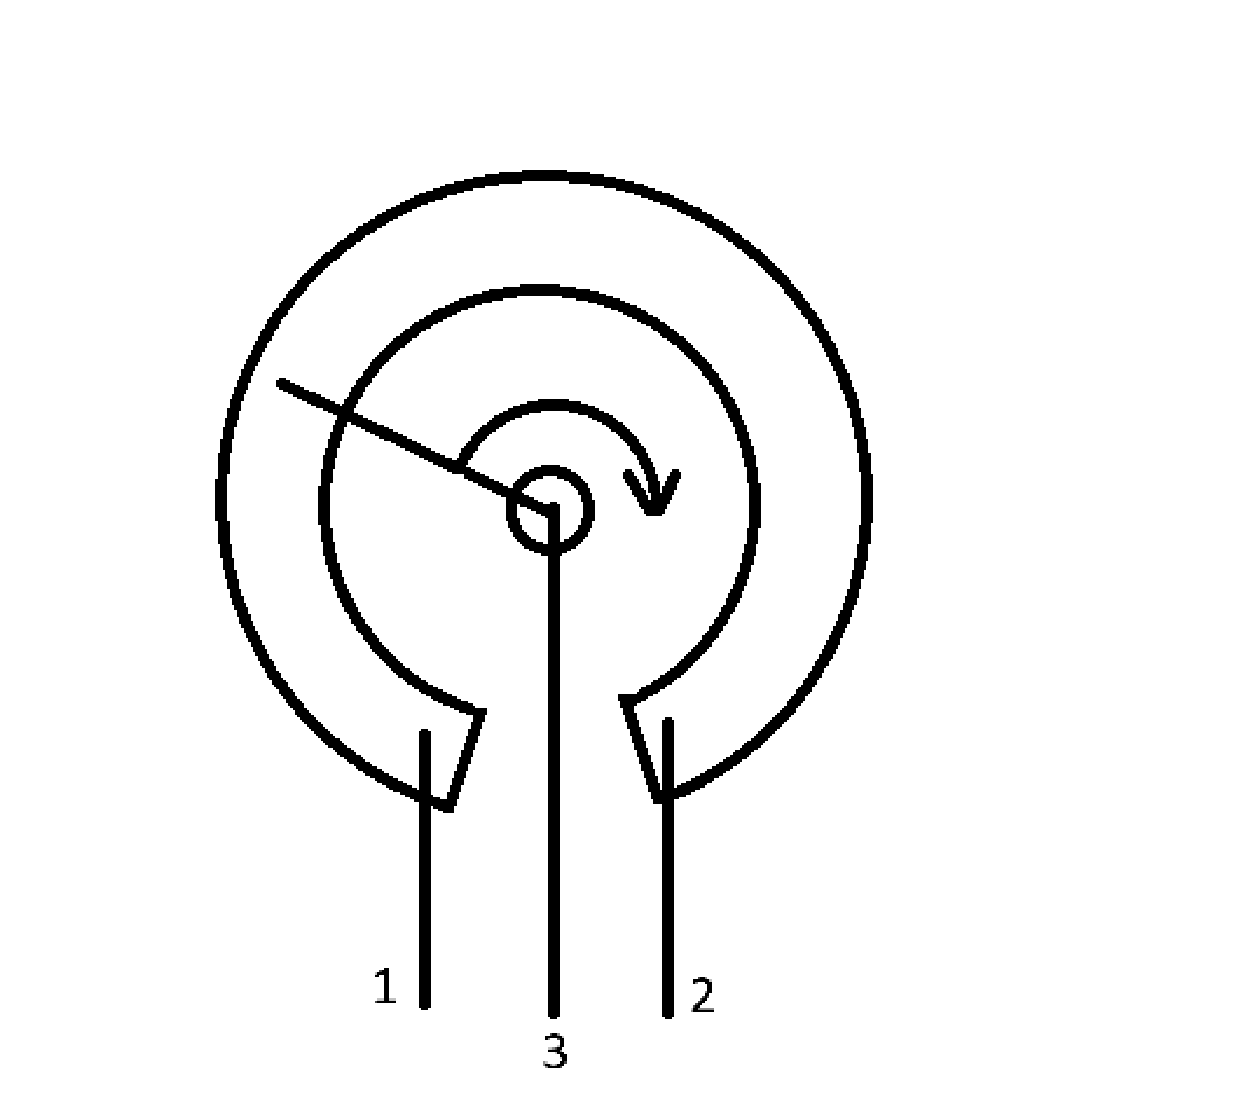
\includegraphics[width = \textwidth]{potterminals.png}
       \label{fig:1}
        \caption{\centering Drawing of a potentiometer with labeled terminals}    
    \end{minipage}
\end{figure}

The resistance between terminals 1 and 2 is constant, while the resistance
between 1 and 3 is determined by equation 1 \cite{report}:
\begin{equation}
    R_{13} = kR
\end{equation}
%ref

Since the potentiometer can be used as a voltage divider, the value of the
potential difference between terminals 1 and 3 will be determined using equation
2\cite{report}:
\begin{equation}
    V_{13} = k V_{tot}
\end{equation} 

When adding a load resistor in parallel to terminals 1 and 3, the voltage across
them can be calculated using equation 3\cite{report}:
%refr
\begin{equation}
    V_{13} = \frac{kR_{L}}{R_{L}+k(1-k)R_P} V
\end{equation}
\section{Methods \& Materials}
All circuits in the experiments were assembled using the provided connection boards. 
The electrical measurements, including voltage and current, were performed using the AM-520 
HVAC multimeter for precision. 
A 10-turn potentiometer with a total resistance of $1 \unit{k\Omega}$ and a resolution of $\Delta k = 0.001$ 
was used to vary resistance and control output voltage. 
The power supply consisted of two 1.5V batteries connected in series. 
Fixed resistors of $1 \unit{k\Omega}$  and $510 \unit{k\Omega}$  were utilized as load resistors, 
along with a decade resistor to provide 
adjustable resistance for certain measurements.


\newpage
\subsection{Experimental Set-Up unloaded potentiometer}
An unloaded potentiometer circuit comprises a voltage source and a potentiometer.
Measurements are taken for both the voltage supplied by the power source
and the potential difference established between terminals 1 and 3. 
In the unloaded potentiometer circuit, measurements are conducted incrementally by varying the parameter 
k from 1 to 0.1. 

Figures 2(a) and 2(b) display both
the electrical diagram, and a picture of the physical set-up of the circuit.

\begin{figure}[!h]
    \centering
    \begin{subfigure}{.5\textwidth}
        \centering
        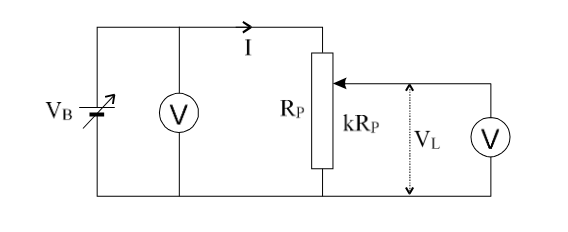
\includegraphics[width=0.8\linewidth]{Unloaded pot circuit.png}
        \label{fig:2a}
        \caption{Circuit diagram of unloaded potentiometer circuit\cite{report}}   
    \end{subfigure}%
    \begin{subfigure}{.5\textwidth}
        \centering
        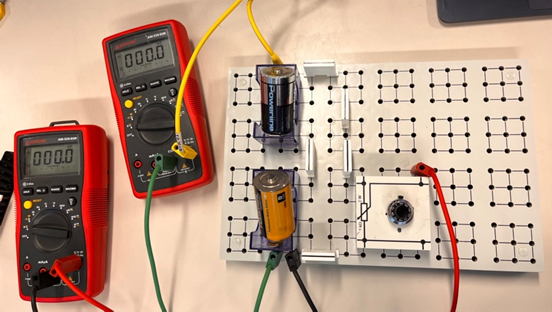
\includegraphics[width = 0.8\linewidth]{unloaded pot picture.png}
        \label{fig2:b}
        \caption{Picture of the unloaded potentiometer circuit}
    \end{subfigure}
    \caption{Electrical schema and physical set-up of the unloaded potentiometer circuit}
\end{figure}
\subsection{Experimental Set-Up with fixed resistor}
The experimental set-up for the second experiment mirrors that of the first, 
with the key distinction being the addition of a load resistor connected in parallel across terminals 1 and 3.
Specifically, a 510 $\Omega$ resistor and a 1 k$\Omega$ resistor are incorporated to introduce varying load conditions.

Figures 3(a) and 3(b) display both the electrical diagram and a picture of the
physical set-up of the circuit.
\begin{figure}[!ht]
    \centering
    \begin{subfigure}{0.5\textwidth}
        \centering
        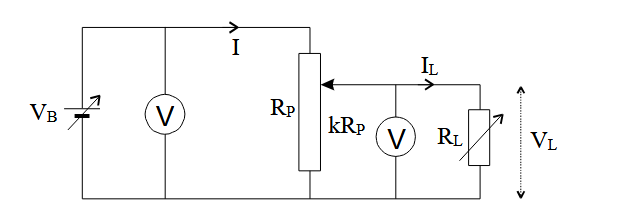
\includegraphics[width = \linewidth]{loaded pot fixed circuit.png}
        \label{fig:3a}
        \caption{Circuit diagram of the loaded \\potentiometer circuit \cite{report}}
    \end{subfigure}%
    \begin{subfigure}{0.5\textwidth}
        \centering
        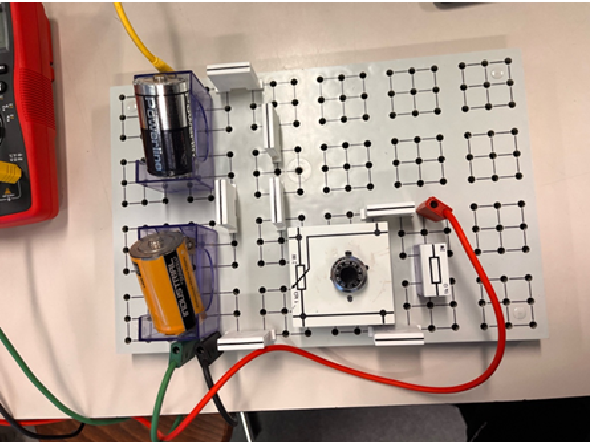
\includegraphics[width = 0.8\linewidth]{loaded pot fixed pic.png}
        \label{fig:3b}
        \caption{Picture of the loaded potentiometer circuit with fixed resistance}        
    \end{subfigure}
    \caption{Electrical schema and physical set-up of the loaded potentiometer with fixed resistance}
\end{figure}
\newpage
\subsection{Experimental Set-Up with fixed load current}
The set-up for the third experiment omits the voltmeter measuring the power
source, replacing it with an ammeter in line with the load resistor. The load
resistor being used becomes a decade resistor.

The experimental flow is also changed, as now with a change in the k-value, the
decade resistor is adjusted in order for the current load to remain the same,
then the resistance of the decade resistor, and the voltage drop is measured.

Figures 4(a), and 4(b) display the circuit diagram and picture of this
experiment.

\begin{figure}[!ht]
    \centering
    \begin{subfigure}{.5\textwidth}
        \centering
        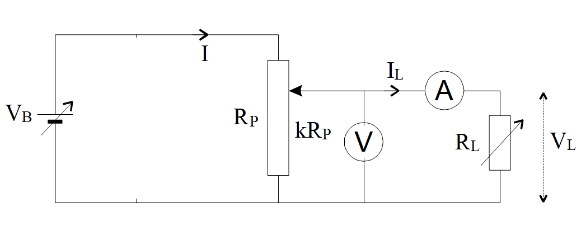
\includegraphics[width = 0.8\linewidth]{fixed current circuit.png}
        \label{fig:4a}
        \caption{Circuit diagram of the constant current load circuit\cite{report}}
        
    \end{subfigure}%
    \begin{subfigure}{.5\textwidth}
        \centering
        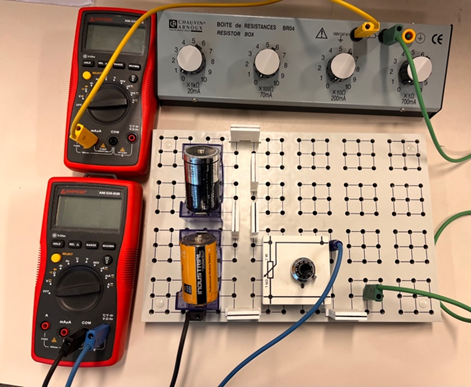
\includegraphics[width = 0.8\linewidth]{fixed currrent picture.png}
        \label{fig:4b}
        \caption{Picture of the constant current load circuit}
    \end{subfigure}
    \caption{Electrical diagram and physical set-up of the constant current load circuit}
\end{figure}
\section{The Unloaded Potentiometer}
\subsection{Measurement Results}
Table 1 presents the measured voltage values $(V_{unloaded})$ corresponding to the different values of the parameter $k$, 
alongside the theoretical voltage values $(V_{expected})$ 
and the associated measurement error $(\Delta V_{unloaded})$ for the unloaded potentiometer circuit.
Additionally, the voltage of the battery was measured and obtained a result of $(V_{cell} = 2.959 \pm 0.028)$ V. 
The calculated error is based on the multimeter's error of reading \cite{noauthor_am-500_2019}.
\begin{table}[!ht]
    \centering
    \label{tab:1}
    \caption{Measured and expected voltage in terms of the parameter k of the potentiometer}
    \begin{tabular}{|c c c c|} 
    \hline
    $k$ & \makecell{$V_{unloaded}$ \\ (V)} & \makecell{$\Delta V_{unloaded}$ \\ (V)} &
    \makecell{$V_{expected}$ \\ (V)}  \\ 
    \hline
    0.1                                       & 0.302      &  0.006          & 0.296      \\
    0.2                                       & 0.594      &  0.006          & 0.592      \\
    0.3                                       & 0.890      &  0.009          & 0.888      \\
    0.4                                       & 1.184      &  0.011          & 1.184      \\
    0.5                                       & 1.481      &  0.013          & 1.480      \\
    0.6                                       & 1.776      &  0.015          & 1.775      \\
    0.7                                       & 2.076      &  0.018          & 2.071      \\
    0.8                                       & 2.365      &  0.020          & 2.367      \\
    0.9                                       & 2.663      &  0.024          & 2.663      \\
    1.0                                       & 2.957      &  0.025          & 2.959      \\
    \hline
    \end{tabular}
    \end{table}
\newpage
\subsection{Graphs}
Figure 5 illustrates the relationship between the measured voltage as a function of the parameter 
k in the unloaded potentiometer circuit.
\begin{figure}[!ht]
    \centering
    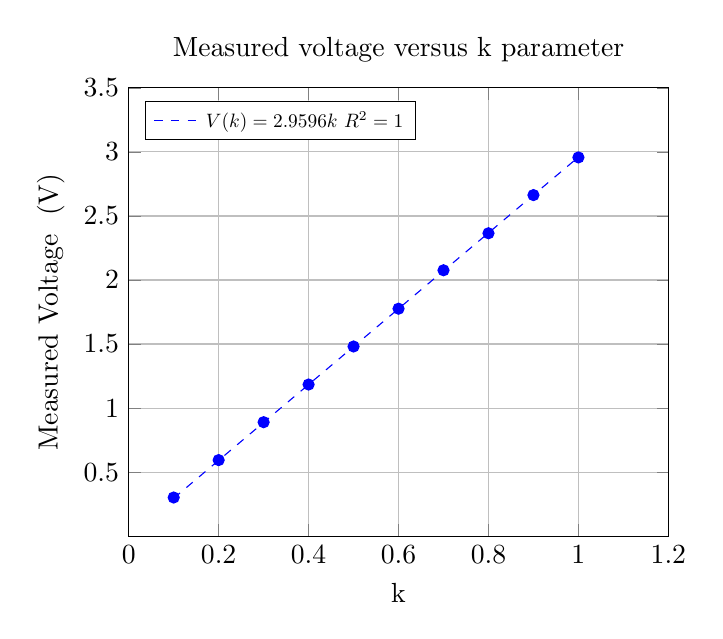
\begin{tikzpicture}
        \begin{axis}[
            title = {Measured voltage versus k parameter},
            xlabel = {k},
            ylabel = {Measured Voltage $ \unit{(V)}$},
            xmin = 0, xmax = 1.2,
            ymin = 0, ymax = 3.5,
            xtick = {0, 0.2, 0.4, 0.6, 0.8, 1.0, 1.2},
            ytick = {0, 0.5, 1, 1.5, 2, 2.5, 3, 3.5},
            ymajorgrids = true,
            xmajorgrids = true,
            legend pos = north west,
            legend style={nodes={scale=0.7}},
            domain = 0.1:1,
            ignore zero = y
        ]
        
        \addplot[blue, samples = 100, dashed]{2.9596*x};
        
        \addplot[only marks, color = blue] coordinates {
            (0.1, 0.302)
            (0.2, 0.594)
            (0.3, 0.89)
            (0.4, 1.184)
            (0.5, 1.481)
            (0.6, 1.776)
            (0.7, 2.076)
            (0.8, 2.365)
            (0.9, 2.663)
            (1.0, 2.957)
        };
        
        \legend{$V(k) = 2.9596k$ $R^2 = 1$}
        
        \end{axis}
    \end{tikzpicture}
    \caption{Measured voltage (V) drop in terms of the k parameter}
    \label{fig:3}
\end{figure}

\subsection{Discussion}
The goal of this experiment was to determine the effect of modifying
the parameter k of the potentiometer on the voltage load. 
The graphical representation of these values in Figure 5 demonstrates
the linear relationship between the k-value and the voltage drop across the potentiometer.
This relationship is consistent with the theoretical formula presented in equation 2.
The slope of the linear relationship, approximately 2.9596, corresponds
to the total voltage supplied by the circuit (approximately 2.960V),
reinforcing the expectation that voltage is directly proportional to the
k-value in an unloaded potentiometer configuration.
Analyzing the difference between measured and expected voltage, 
the results show strong agreement,
with discrepancies falling within the calculated measurement error. 
These minor deviations can be attributed to potential inaccuracies
in measurement or the inherent precision limits of the multimeter.
Furthemore, the total voltage supplied by the circuit 
expected from the theoretical formula is strongly related to the one recorded
by measuring the power source $(V_{cell} = 2.959 \pm 0.028)$, further confirming the accuracy of the data.
\newpage
\section{Potentiometer loaded with fixed resistor}
\subsection{Measurement results}
Table 2 presents the measurements for k,
including the unloaded potentiometer value and the values corresponding to both loads,
$1 k\Omega$ as load 1 and $510~\Omega$ as load 2.
The table provides both the measured $V_{L1}$ and $V_{L2}$ values, and theoretical values $V_{L1t}$ and $V_{L2t}$, 
along with the calculated percent deviations $PD_1$ and $PD_2$.
\begin{table}[!ht]
    \centering
    \label{tab:2}
    \caption{Measured and theoretical voltage for $1 \unit{k\Omega}$ and $510\unit{\Omega}$
    load values in terms of k}
    \begin{tabular}{|c c c c c c c c|} 
    \hline
    $k$ & \makecell{$V_{unloaded}$\\ (V)} & \makecell{$V_{L1}$\\ (V)} & 
    \makecell{$V_{L1t}$\\ (V)} & \makecell{$PD_{1}$\\ (\%)}  & \makecell{$V_{L2}$\\ (V)} &
    \makecell{$V_{L2t}$\\ (V)}
    & \makecell{$PD_2$ \\ (\%)}   \\ 
    \hline
    0.1     & 0.302    & 0.274  & 0.271                & 9.27   & 0.253  & 0.254               & 16.23  \\
    0.2     & 0.594    & 0.514  & 0.510                & 13.47  & 0.451  & 0.457               & 24.07  \\
    0.3     & 0.890    & 0.739  & 0.734                & 16.97  & 0.628  & 0.640               & 29.44  \\
    0.4     & 1.184    & 0.957  & 0.954                & 19.17  & 0.809  & 0.820               & 31.67  \\
    0.5     & 1.481    & 1.184  & 1.183                & 20.05  & 0.993  & 1.012               & 32.95  \\
    0.6     & 1.776    & 1.433  & 1.431                & 19.31  & 1.210  & 1.230               & 31.87  \\
    0.7     & 2.076    & 1.717  & 1.712                & 17.29  & 1.470  & 1.493               & 29.19  \\
    0.8     & 2.365    & 2.039  & 2.040                & 13.78  & 1.801  & 1.828               & 23.85  \\
    0.9     & 2.663    & 2.448  & 2.443                & 8.07   & 2.268  & 2.284               & 14.83  \\
    1.0     & 2.957    & 2.952  & 2.959                & 0.17   & 2.948  & 2.959               & 0.30   \\
    \hline
    \end{tabular}
    \end{table}
\subsection{Graphs}
Figure 6 illustrates the relationship between the voltage across the load resistor
and the parameter 
k, comparing the experimental results with the 
corresponding theoretical values. 
Additionally, it presents the voltage drop across the unloaded potentiometer for reference.
\begin{figure}[!ht]
    \centering
    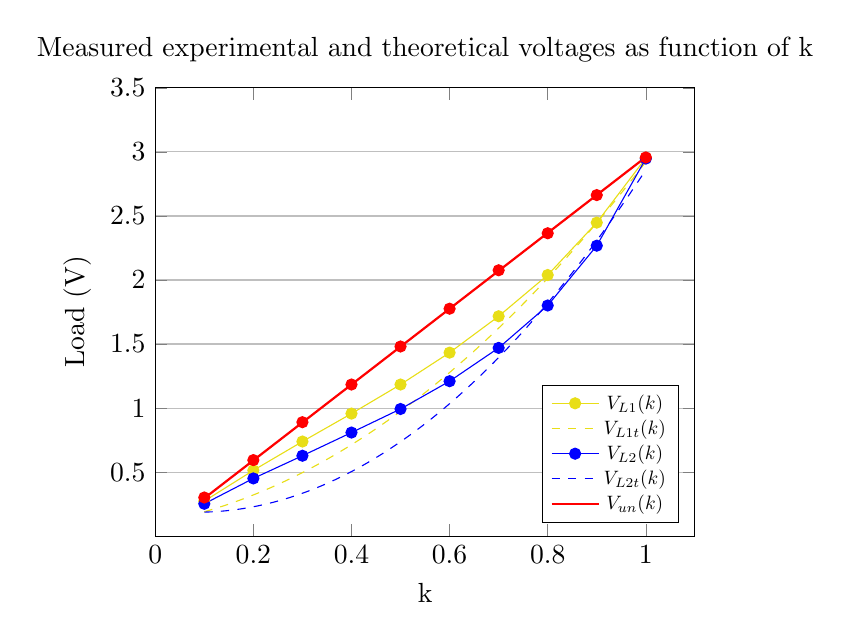
\begin{tikzpicture}
        \begin{axis}[
            title = {Measured experimental and theoretical voltages as function of k}, 
            legend pos = south east, 
            legend style={nodes={scale=0.7}}, 
            ymajorgrids = true, 
            domain = 0.1:1, 
            xmin = 0, xlabel = k, xtick = {0, 0.2, 0.4, 0.6, 0.8, 1.0, 1.2}, ymin = 0, ymax = 3.5, ytick = {0, 0.5, 1, 1.5, 2, 2.5, 3, 3.5}, ylabel = Load$ \unit{(V)}$, ignore zero = y, ]
        
        %\addplot[black!10!yellow, thick, samples = 100]{1.52*(x^2) + 1.157*x +0.2};
        \addplot  [mark = *, color = black!10!yellow] coordinates {
            (0.1,	0.274)
            (0.2,	0.514)
            (0.3,	0.739)
            (0.4,	0.957)
            (0.5,	1.184)
            (0.6,	1.433)
            (0.7,	1.717)
            (0.8,	2.039)
            (0.9,	2.448)
            (1.0,	2.952)

            
        };
         
        \addplot[black!10!yellow, thin, samples = 100, dashed]{2.15*(x^2) + 0.67 * x +
        0.102};
        %\addplot[blue, thick, samples=100]{2.49*(x^2) + 0.39};
        \addplot  [mark = *,  color = blue] coordinates {
            (0.1,	0.253)
            (0.2,	0.451)
            (0.3,	0.628)
            (0.4,	0.809)
            (0.5,	0.993)
            (0.6,	1.21)
            (0.7,	1.47)
            (0.8,	1.801)
            (0.9,	2.268)
            (1.0,	2.948)
            

            
        };
        \addplot[blue, thin, samples=100, dashed]{3.19*(x^2) - 0.54 * x + 0.21};
        \addplot[red, samples = 100, thick]{2.9596*x};
        
        \addplot[only marks, color = red] coordinates {
            (0.1, 0.302)
            (0.2, 0.594)
            (0.3, 0.89)
            (0.4, 1.184)
            (0.5, 1.481)
            (0.6, 1.776)
            (0.7, 2.076)
            (0.8, 2.365)
            (0.9, 2.663)
            (1.0, 2.957)
        };
        \legend{$V_{L1}(k)$, $V_{L1t}(k)$,$V_{L2}(k)$, $V_{L2t}(k)$,$V_{un}(k)$ }
        \end{axis}
    \end{tikzpicture}
    \caption{\centering Measured experimental and theoretical voltages in fixed resistor circuit for 
            load 1 and load 2 as a function of k}
    \label{fig:5}
\end{figure}
\newpage
Furthermore, Figure 7 displays the relationship between percent deviation
and the k parameter
\begin{figure}[!ht]
    \centering
    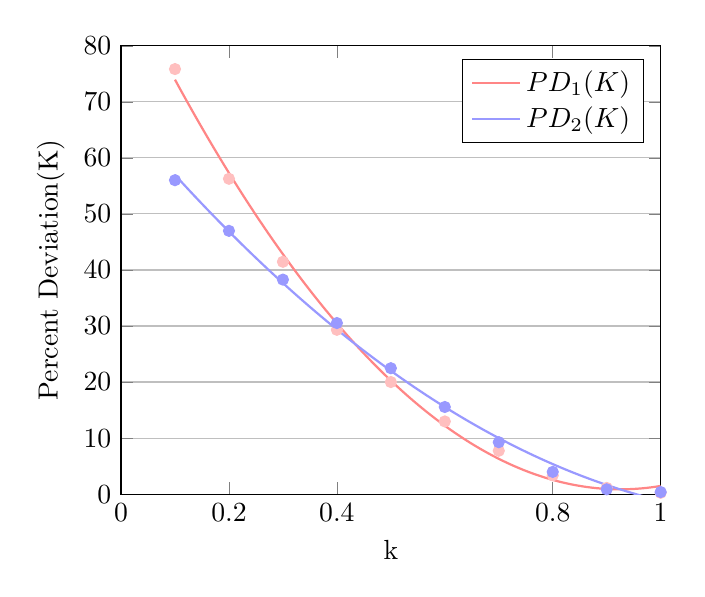
\begin{tikzpicture}
        \begin{axis}[legend pos = north east, legend style={nodes={scale=1}},
        ymajorgrids = true, domain = 0.1:1, xmin = 0, xmax = 1, ymin = 0, ymax =
        80, xlabel = k, xtick = {0, 0.2, 0.4, 0.8, 1}, ytick = {0, 10, 20, 30,
        40, 50, 60, 70, 80}, ylabel = Percent Deviation(K)]
        \addplot[red!30!pink, thick, samples = 100]{107.36*(x^2) - 198.65*x +92.75};
        \addplot[only marks, color = pink, forget plot] 
        coordinates {
            (0.1,	75.85)
            (0.2,	56.27)
            (0.3,	41.46)
            (0.4,	29.32)
            (0.5,	20.00)
            (0.6,	12.97)
            (0.7,	7.74)
            (0.8,	3.35)
            (0.9,	1.11)
            (1.0,	0.24)
             
        };
        \addplot[white!60!blue, thick, samples = 100]{45.56*(x^2) - 114.72*x + 67.98};
        \addplot[only marks, color = white!60!blue, forget plot] 
        coordinates{    
        (0.1,	56.02)
        (0.2,	46.98)
        (0.3,	38.28)
        (0.4,	30.53)
        (0.5,	22.47)
        (0.6,	15.55)
        (0.7,	9.27)
        (0.8,	3.97)
        (0.9,	0.86)
        (1.0,	0.37)
        };
        \legend{$PD_ 1(K)$,$PD_2(K)$}
        \end{axis}
    \end{tikzpicture}
    \label{fig:6}
    \caption{Percent deviation in terms of k}
\end{figure}
\subsection{Calculations}
To calculate the theoretical load, equation 3 is used. Using k = 0.5 and $R_L =
543\unit{\Omega}$ the following calculation is made:
\begin{gather*}
    V_{13} = \frac{kR_L}{R_L + k(1-k) R_P} \cdot V = \frac{0.5 \cdot 543}{543 + 0.5(1-0.5)1001} \cdot 2.959 = 1.012\unit{V}
\end{gather*}
Using the user manual of the multimeter, $\Delta V, ~\Delta R_L, ~\Delta R_P$ can
be determined\cite{noauthor_am-500_2019}:
\begin{gather}
    \Delta R = \frac{R}{100} + 2LSD\\
    \Delta V = \frac{0.8 V}{100} + 1LSD\\
    \Delta R_L = \frac{543}{100} + 2LSD = 5.46\unit{\Omega} \nonumber \\
    \Delta R_P = \frac{1001}{100} + 2LSD = 10.02\unit{\Omega} \nonumber \\
    \Delta V_P = \frac{0.8 \cdot 2.959}{100} + LSD = 0.00616\unit{V} \nonumber
\end{gather} 
To calculate the error values of $V_{th}$, the following formula is used \cite{unc}:
\begin{equation}
    \frac{\Delta V_{th}}{V_{th}} = \sqrt{\left( \frac{\Delta V_P}{V_P}\right) ^2 + \left( \frac{\Delta R_P}{R_P} \right) ^ 2 + \left( \frac{\Delta R_L}{R_L} \right) ^2}
\end{equation}
Calculating this value for $k = 0.5$, $R_L = 543\unit{\Omega}$:
\[ \Delta V_{th} = 0.77 \sqrt{\left( \frac{0.00616}{2.959} \right) ^ 2 + \left(
\frac{10.02}{1001} \right) ^2 + \left(\frac{5.46}{543} \right) ^2 } = 0.011
\unit{V} \]
The error for the measured voltage will be calculated using equation 5:
\[ \Delta V = \frac{0.8 \cdot 0.993}{100} + LSD = 0.0109\unit{V} \]
Therefore, in standard notation the results for $V_{th}$ and $V_L$ are:
\begin{gather*}
    V_{th} = (1.012 \pm 0.02) \unit{V}\\
    V_L = (0.993 \pm 0.02) \unit{V}
\end{gather*}

\subsection{Discussion}
This experiment aimed to analyze the voltage across the potentiometer when loaded with parallel resistors 
of $1 \unit{k\Omega}$ and $510\unit{\Omega}$. 
According to Figure 6, the relationship between the k-value and load voltage follows a non-linear trend, 
especially at lower k-values. Additionally, Figure 7 highlights that the percentage deviations show a more 
pronounced variation at lower k-values. For instance, at a k-value of 0.5, the percentage deviation was 20.05\%
for the $1 \unit{k\Omega}$ load and 32.95\% for the $510\unit{\Omega}$ load. 
These values suggest potential systematic errors, possibly due to human intervention or equipment inconsistencies at lower values.

These deviations are notable but fall within a plausible range given the potential loading effects and measurement uncertainties. 
As the k-value increased, the percentage deviation decreased, with minimal deviations observed at k = 1.0, 
where deviations were 0.17\% for the $1 \unit{k\Omega}$ load and 0.30\% for the $510\unit{\Omega}$ load.

Such deviations can be attributed to loading effects, 
the influence of connection resistance, and inherent limitations in the precision of the multimeter. 
Despite these discrepancies, the general trend of the measured values aligns with theoretical expectations. 
The similarity in the overall behaviour of the experimental and theoretical graphs (Figure 6) 
confirms that the theoretical model accurately represents the system's behavior, 
particularly at higher k-values where deviations diminish.

\section{Potentiometer with fixed load current}
\subsection{Measurement results}
Table 3 displays the values for $V_{th}$, $V_{L}$, $PD_1$, $PD_2$, and
$V_{unloaded}$:
\begin{table}[!ht]
    \centering
    \label{tab:3}
    \caption{Measured and calculated values for the third experiment}
    \begin{tabular}{|c|c|c|c|c|c|c|c|} 
    \hline
    $K$ & \makecell{$V_{unloaded}$ \\ $\unit{V}$} & \makecell{$V_{L_1}$ \\
    $\unit{V}$} & \makecell{$V_{th_1}$ \\ $\unit{V}$} &
    \makecell{$PD_1$\\$\unit{\%}$}      & \makecell{$V_{L_2}$ \\ $\unit{V}$} &
    \makecell{$V_{th_2}$ \\ $\unit{V}$} & \makecell{$PD_1$ \\ $\unit{\%}$}         \\ 
    \hline
    0.1     & 0.302      & 0.108  & 0.116            & 64.24    & N/A    & N/A             & N/A    \\
    0.2     & 0.594      & 0.257  & 0.271            & 56.73    & N/A    & N/A             & N/A    \\
    0.3     & 0.890      & 0.431  & 0.467            & 51.57    & 0.029  & 0.046           & 96.74  \\
    0.4     & 1.184      & 0.654  & 0.703            & 44.76    & 0.194  & 0.222           & 83.61  \\
    \textbf{0.5}     & \textbf{1.481}      & \textbf{0.968}  & \textbf{0.979}             & \textbf{34.64} & 0.430   & 0.478             & 70.97  \\
    0.6     & 1.776      & 1.214  & 1.294            & 31.64    & 0.755  & 0.813           & 57.49  \\
    0.7     & 2.076      & 1.554  & 1.650            & 25.14    & 1.156  & 1.230           & 44.32  \\
    0.8     & 2.365      & 1.925  & 2.047            & 18.60    & 1.639  & 1.726           & 30.70  \\
    0.9     & 2.663      & 2.340  & 2.482            & 12.13    & 2.192  & 2.302           & 17.69  \\
    1       & 2.957      & 2.786  & 2.959            & 5.78     & 2.838  & 2.959           & 4.02   \\
    \hline
    \end{tabular}
    \end{table}
\subsection{Graphs}
Figure 8 represents the load voltages, both theoretical and measured, in terms
of the k-value:
\begin{figure}[!ht]
    \centering
    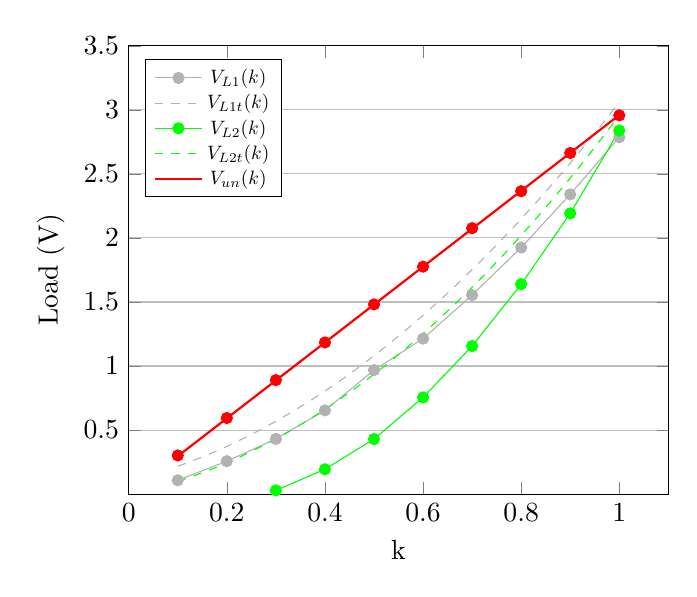
\begin{tikzpicture}
        \begin{axis}[legend pos = north west, legend style={nodes={scale=0.7}}, ymajorgrids = true, domain = 0.1:1, xmin = 0, xlabel = k, xtick = {0, 0.2, 0.4, 0.6, 0.8, 1.0, 1.2}, ymin = 0, ymax = 3.5, ytick = {0, 0.5, 1, 1.5, 2, 2.5, 3, 3.5}, ylabel = Load$ \unit{(V)}$, ignore zero = y, ]
        
        %\addplot[black!10!yellow, thick, samples = 100]{1.52*(x^2) + 1.157*x +0.2};
        \addplot  [mark = *, color = black!30!white] coordinates {
            (0.1,	0.108)
            (0.2,	0.257)
            (0.3,	0.431)
            (0.4,	0.654)
            (0.5,	0.968)
            (0.6,	1.214)
            (0.7,	1.554)
            (0.8,	1.925)
            (0.9,	2.34)
            (1,	2.786)
            

            
        };
         
        \addplot[black!30!white, thin, samples = 100, dashed]{2.004*(x^2) + 0.955 * x +
        0.102};
        %\addplot[blue, thick, samples=100]{2.49*(x^2) + 0.39};
        \addplot  [mark = *,  color = green] coordinates {
            (0.3,	0.029)
            (0.4,	0.194)
            (0.5,	0.43)
            (0.6,	0.755)
            (0.7,	1.156)
            (0.8,	1.639)
            (0.9,	2.192)
            (1,	2.838)
            
            

            
        };
        \addplot[green, thin, samples=100, dashed]{2.172*(x^2) + 0.787 * x};
        \addplot[red, samples = 100, thick]{2.9596*x};
        
        \addplot[only marks, color = red, forget plot] coordinates {
            (0.1, 0.302)
            (0.2, 0.594)
            (0.3, 0.89)
            (0.4, 1.184)
            (0.5, 1.481)
            (0.6, 1.776)
            (0.7, 2.076)
            (0.8, 2.365)
            (0.9, 2.663)
            (1.0, 2.957)
        };
        \legend{$V_{L1}(k)$, $V_{L1t}(k)$,$V_{L2}(k)$, $V_{L2t}(k)$,$V_{un}(k)$ }
        \end{axis}
    \end{tikzpicture}
    \label{fig:8}
    \caption{Loads in terms of k}
\end{figure}
\newpage
Figure 9 represents the two percent deviations in terms of the k-value.
\begin{figure}[!ht]
    \centering
    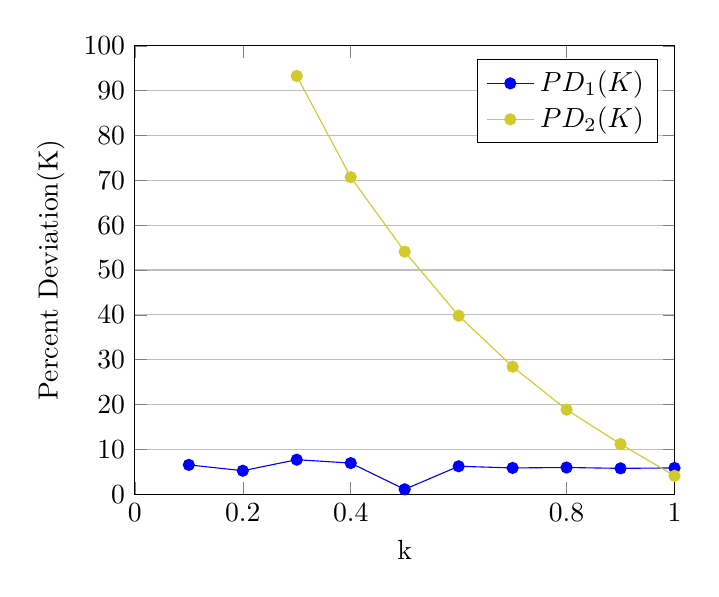
\begin{tikzpicture}
        \begin{axis}[legend pos = north east, legend style={nodes={scale=1}},
        ymajorgrids = true, domain = 0.1:1, xmin = 0, xmax = 1, ymin = 0, ymax =
        100, xlabel = k, xtick = {0, 0.2, 0.4, 0.8, 1}, ytick = {0, 10, 20, 30,
        40, 50, 60, 70, 80,90,100}, ylabel = Percent Deviation(K)]
        %\addplot[red!30!pink, thick, samples = 100]{107.36*(x^2) - 198.65*x +92.75};
        \addplot[mark = *, color = blue] 
        coordinates {
            (0.1,	6.525878484)
            (0.2,	5.222009146)
            (0.3,	7.681103543)
            (0.4,	6.922463851)
            (0.5,	1.073071027)
            (0.6,	6.214270264)
            (0.7,	5.844431249)
            (0.8,	5.939723243)
            (0.9,	5.74929312)
            (1,	5.846569787)
            
             
        };
        %\addplot[white!60!blue, thick, samples = 100]{45.56*(x^2) - 114.72*x + 67.98};
        \addplot[mark = *, color = black!20!yellow] 
        coordinates{    
            (0.3,	93.28050419)
            (0.4,	70.70902283)
            (0.5,	54.08435665)
            (0.6,	39.79842439)
            (0.7,	28.42902958)
            (0.8,	18.84853046)
            (0.9,	11.16946694)
            (1.0,	4.089219331)
            
        };
        \legend{$PD_ 1(K)$,$PD_2(K)$}
        \end{axis}
    \end{tikzpicture}
    \label{fig:9}
    \caption{Percent deviation in terms of k}
\end{figure}
\subsection{Calculations}
Due to the variable resistance of the decade resistor, $R_L$ at $ k = 0.5$ will
be $480\unit{\Omega}$.

Firstly, using equation 3, the theoretical load can be calculated:
\[ V_L = \frac{0.5 \cdot 480}{480 + 0.5(1-0.5)1001} \cdot 3 = 0.979\unit{V}\]
Using the values highlighted in table 3, the sample error calculations can be made.

Using equations 4 and 5, the calculations for $\Delta R$, and $\Delta V$ are:
\begin{gather*}
    \Delta R_L = \frac{480}{100} + 2LSD = 4.8\unit{\Omega}\\
    \Delta R_P = 10.02\unit{\Omega}\\
    \Delta V_L = \frac{0.08 \cdot 0.968}{100} + 0.008 = 0.01557\unit{V}
\end{gather*}
Using equation 6, the error for the theoretical value can be found:
\[ \Delta V_{th} = 0.979 \sqrt{\left( \frac{0.01557}{0.968} \right) ^2 + \left(
\frac{10.02}{1001} \right) ^2 + \left( \frac{4.8}{480} \right) ^2} = 0.021
\unit{V}\]

Therefore the load values in standard notation are:
\begin{gather*}
    V_{th} = (0.979 \pm 0.021)\unit{V}\\
    V_L = (0.968 \pm 0.016)\unit{V}
\end{gather*}
\subsection{Discussion}
In this experiment, a constant current load was analyzed.
Significant deviations from theoretical predictions were observed, especially at lower k-values. 
Firstly, the values for the fixed 4mA current did not coincide with the theoretical values. 
This is likely due to the effect of the internal resistance of the batteries on the rest of the circuit. 
Typical batteries have an internal resistance of around $0.2 \unit{\Omega}$ at room temperature \cite{ir}. 
Thus, when decreasing both the potentiometer's k-value and the decade resistor, 
the internal resistance had a greater impact since the external resistances were smaller.
Internal resistance is also likely the cause of the discrepancy in the first current load. 
However, since the external resistances were larger, the overall effect of internal resistance was less pronounced.

Furthermore, the percentage deviation discrepancies could be attributed to the circuit construction method. 
Since the connections were more exposed compared to a traditional circuit, 
external interference may have skewed the results. 
This suggests that ensuring better connections and minimizing external interference would enhance measurement accuracy.
\section{Conclusion}
This study explored the relationship between the potentiometer's k-value and the resulting voltage in various circuit configurations. 
The unloaded potentiometer demonstrated a clear linear correlation, aligning well with theoretical expectations.
When introducing fixed resistors, deviations were noted, particularly at lower k-values, due to loading effects. 
In the fixed load current experiment, internal battery resistance and circuit construction impacted measurement accuracy. 
While theoretical predictions provided a solid foundation, practical factors introduced measurable deviations, 
emphasizing the importance of considering real-world conditions in experimental analysis.
\section{Bibliography}
\bibliographystyle{IEEEtran}
\bibliography{ELECTRICITY_2}
\end{document}